LLVM IR是要优化和编译程序的另一种形式。然而,它的结构不同于C/C++等普通编程语言。LLVM IR以分层的方式组织。这个层次结构中的层次——从顶部开始计算——是模块、函数、基本块和指令。下面的图表显示了它们的结构:

\hspace*{\fill} \\ %插入空行
\begin{center}
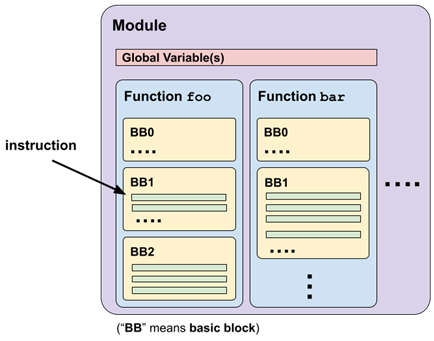
\includegraphics[width=0.8\textwidth]{content/3/chapter10/images/1.png}\\
图10.1 - LLVM IR的层级结构
\end{center}

一个\textbf{模块}代表一个翻译单元——通常是一个源文件。每个模块可以包含多个\textbf{函数}(或全局变量)。每个都包含一个\textbf{基本块}列表,每个基本块包含一个\textbf{指令}列表。

\begin{tcolorbox}[colback=blue!5!white,colframe=blue!75!black, fonttitle=\bfseries,title=简要介绍——基本块]	
\hspace*{0.7cm}基本块表示一个只有一个入口和一个出口的指令列表。换句话说,如果执行一个基本块,控制流需要保证遍历块中的每一条指令。
\end{tcolorbox}

了解LLVM IR的结构后,让我们看一个LLVM IR的例子。假设我们有下面的C代码\texttt{foo.c}:

\begin{lstlisting}[style=styleCXX]
int foo(int a, int b) {
	return a > 0? a – b : a + b;
}
\end{lstlisting}

我们可以使用下面的\texttt{clang}命令来生成文本形式的LLVM IR:

\begin{tcblisting}{commandshell={}}
$ clang -emit-llvm -S foo.c
\end{tcblisting}

结果将放到\texttt{foo.ll}文件中。下图显示了其部分内容,并对相应的IR单元进行了注释:

\hspace*{\fill} \\ %插入空行
\begin{center}
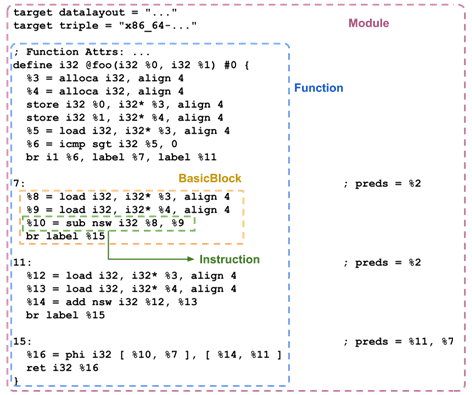
\includegraphics[width=0.8\textwidth]{content/3/chapter10/images/2.png}\\
图10.2 - foo.ll中的部分内容,使用相应的IR单元进行标注
\end{center}

在文本形式中,指令通常以以下格式呈现:

\begin{tcblisting}{commandshell={}}
<result> = <operator / op-code> <type>, [operand1, operand2, …]
\end{tcblisting}

例如,假设我们有以下指令:

\begin{tcblisting}{commandshell={}}
%12 = load i32, i32* %3
\end{tcblisting}

在这里,\texttt{\%12}是结果值,\texttt{load}是操作码,\texttt{i32}是该指令的数据类型,\texttt{\%3}是唯一的操作数。

除了文本表示之外,LLVM IR中的几乎每个组件都有一个名称相同的C++类对应项,例如:函数和基本块分别由\texttt{Function}和\texttt{BasicBlock} C++类简单地表示。

不同种类的指令由类表示,这些类都由\texttt{Instruction}类派生,例如:\texttt{BinaryOperator}类表示二进制操作指令,而\texttt{Returnst}类表示返回语句。稍后,我们将更详细地介绍\texttt{Instruction}及其子类。

图10.1所示的层次结构是LLVM IR的具体结构,这就是它们在内存中的存储方式。在此基础上,LLVM还提供了其他逻辑结构来查看不同IR单元的关系。它们通常对具体的结构进行评估,并作为辅助数据结构存储或作为分析结果处理。以下是LLVM中最重要的一些内容:

\begin{itemize}
\item \textbf{控制流图(CFG)}:这是一种组织成基本块的图结构,以显示控制流关系。图中的顶点代表基本块,而边代表单个控制流传输路径。

\item \textbf{循环}:这表示我们熟悉的循环,它由多个基本块组成,至少有一条后边——一条返回父顶点或祖先顶点的控制流边。我们将在本章的最后一节中更详细地进行讨论。

\item \textbf{调用图}:与CFG类似,调用图也显示了控制流传输,但是顶点变成了单独的函数,而边变成了函数调用关系。
\end{itemize}

下一节中,我们将了解如何在具体和逻辑结构中迭代不同的IR单元。

\subsubsubsection{10.2.1\hspace{0.2cm}迭代不同的IR单元}

迭代IR单元——基本块或指令——对于LLVM IR开是必不可少。这通常是我们在许多转换或分析算法中必须完成的第一步——扫描整个代码,并找到一个感兴趣的区域,以便应用某些测量工具。本节中,将了解如何迭代不同IR单元。我们将讨论以下内容:

\begin{itemize}
\item 迭代指令
\item 迭代基本块
\item 迭代调用图
\item 了解GraphTraits
\end{itemize}

让我们从讨论如何迭代指令开始。

\subsubsubsection{10.2.2\hspace{0.2cm}迭代指令}

指令是LLVM IR中最基本的元素之一,通常表示程序中的单个操作,例:如算术操作或函数调用。遍历单个基本块或函数中的所有指令是大多数程序分析和编译器优化的基础。

要遍历一个基本块中的所有指令,只需要在块上使用一个简单的for-each循环:

\begin{lstlisting}[style=styleCXX]
// `BB` has the type of `BasicBlock&`
for (Instruction &I : BB) {
	// Work on `I`
}
\end{lstlisting}

我们可以用两种方法遍历函数中的所有指令。首先,在访问指令之前,可以遍历函数中的所有基本块。下面是一个例子:

\begin{lstlisting}[style=styleCXX]
// `F` has the type of `Function&`
for (BasicBlock &BB : F) {
	for (Instruction &I : BB) {
		// Work on `I`
	}
}
\end{lstlisting}

其次,可以利用一个名为\texttt{inst\_iterator}的程序。下面是一个例子:

\begin{lstlisting}[style=styleCXX]
#include "llvm/IR/InstIterator.h"
…
// `F` has the type of `Function&`
for (Instruction &I : instructions(F)) {
	// Work on `I`
}
\end{lstlisting}

使用前面的代码,可以检索这个函数中的所有指令。

\hspace*{\fill} \\ %插入空行
\noindent
\textbf{观察指令}

在很多情况下,我们希望对一个基本块或函数中的不同类型的指令应用有不同的处理方法。例如,我们有以下代码:

\begin{lstlisting}[style=styleCXX]
for (Instruction &I : instructions(F)) {
	switch (I.getOpcode()) {
		case Instruction::BinaryOperator:
		// this instruction is a binary operator like `add` or `sub`
		  break;
		case Instruction::Return:
		// this is a return instruction
		  break;
		…
	}
}
\end{lstlisting}

不同种类的指令由来自\texttt{Instruction}的(不同)类进行建模。因此,一个\texttt{Instruction}实例可以表示它们中的任何一个。前面代码片段中显示的\texttt{getOpcode}方法可以为您提供唯一的令牌——即给定代码中的\texttt{Instruction::BinaryOperator}和\texttt{Instruction::Return}——展示有关底层类的信息。然而,如果想处理派生类(在本例中为\texttt{Returnst})实例,而不是“原始”\texttt{Instruction},则需要进行一些类型转换。

LLVM提供了一种更好的方法来实现这种访问模式——\texttt{Instvisitor}。\texttt{InstVisitor}是一个类,每个成员方法都是特定指令类型的回调函数。可以在继承了\texttt{InstVisitor}类后定义自己的回调函数。例如,下面的代码:

\begin{lstlisting}[style=styleCXX]
#include "llvm/IR/InstVisitor.h"
class MyInstVisitor : public InstVisitor<MyInstVisitor> {
	void visitBinaryOperator(BinaryOperator &BOp) {
		// Work on binary operator instruction
		…
	}
	void visitReturnInst(ReturnInst &RI) {
		// Work on return instruction
		…
	}
};
\end{lstlisting}

这里显示的每个\texttt{visitXXX}方法都是特定指令类型的回调函数。请注意,我们没有覆盖这些方法(没有覆盖关键字附加到方法)。而且,\texttt{InstVisitor}不是为所有指令类型定义回调函数,而是允许定义那些我们感兴趣的指令类型。

当定义\texttt{MyInstVisitor}后,就可以简单地创建它的实例,并调用\texttt{visit}方法来启动访问流程。以下面的代码为例:

\begin{lstlisting}[style=styleCXX]
// `F` has the type of `Function&`
MyInstVisitor Visitor;
Visitor.visit(F);
\end{lstlisting}

还有\texttt{Instruction}、\texttt{BasicBlock}和\texttt{Module}的\texttt{visit}方法。

\begin{tcolorbox}[colback=blue!5!white,colframe=blue!75!black, fonttitle=\bfseries,title=基本块和指令的排序]	
\hspace*{0.7cm}我们在本节中介绍的所有技能都假设,基本块的排序或访问指令(这不是主要关注点)。然而,重要的是要知道\texttt{Function}不会以特定的线性顺序存储,或迭代其闭环的\texttt{BasicBlock}实例。我们将展示如何以各种有意义的顺序,是如何遍历所有基本块的。
\end{tcolorbox}

在此基础上,了解了从基本块或函数迭代指令的几种方法。现在,让我们了解一下如何在函数中迭代基本块。

\subsubsubsection{10.2.3\hspace{0.2cm}迭代基本块}

前一节中,了解了如何使用简单的for循环迭代函数的基本块。然而,开发人员只能以这种方式接收任意顺序的基本块——这种顺序既没有给定执行顺序,也没有给定块之间的控制流信息。本节中,我们将展示如何以更有意义的方式迭代基本块。

基本块是表达函数控制流的重要元素,可以用有向图表示——即CFG。为了让你对典型的CFG有一个具体的了解,我们利用\texttt{opt}工具中的特性。假设你有一个LLVM IR文件\texttt{foo.ll},可以使用以下命令以Graphviz格式打印出每个函数的CFG:

\begin{tcblisting}{commandshell={}}
$ opt -dot-cfg -disable-output foo.ll
\end{tcblisting}

这个命令将为\texttt{foo.ll}中的每个函数生成一个\texttt{.dot}文件。

\begin{tcolorbox}[colback=blue!5!white,colframe=blue!75!black, fonttitle=\bfseries,title=.dot文件可能会被隐藏]	
\hspace*{0.7cm}CFG的\texttt{.dot}文件中每个函数的文件名通常以点字符('.')开头。在Linux/Unix系统上,这有将会让文件隐藏起来,不能使用普通的\texttt{ls}看到。因此,需要使用\texttt{ls -a}才能来显示这些文件。
\end{tcolorbox}

每个texttt{.dot}文件包含该函数的CFG的Graphviz表示。Graphviz是表示图形的通用文本格式,人们通常在研究texttt{.dot}文件之前将其转换为其他(图像)格式,例如:使用下面的命令,可以将texttt{.dot}文件转换为PNG图像文件,以直观地显示图形:

\begin{tcblisting}{commandshell={}}
$ dot -Tpng foo.cfg.dot > foo.cfg.png
\end{tcblisting}

下图有两个示例:

\hspace*{\fill} \\ %插入空行
\begin{center}
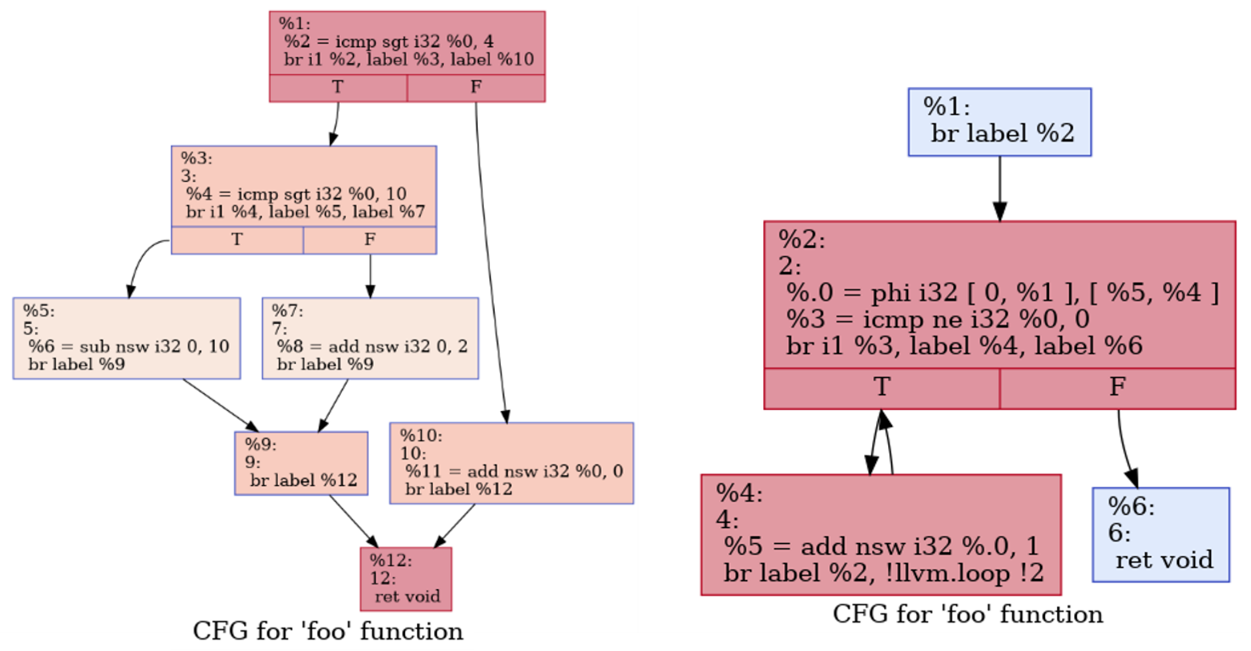
\includegraphics[width=0.9\textwidth]{content/3/chapter10/images/3.png}\\
图10.3 -左:包含分支的函数的CFG;右:CFG用于包含循环的函数
\end{center}

上图的左边显示了包含几个分支的函数的CFG,右边显示了一个包含单循环的函数的CFG。

现在,我们知道基本块组织成一个有向图——也就是CFG。可以迭代这个CFG,使它沿着边和节点吗?LLVM通过提供四种不同方式迭代图的实用工具来回答这个问题:拓扑顺序、深度优先(本质上是做DFS)、广度优先(本质上是做BFS)和强连接组件(SCCs)。我们将在下面的小节中学习如何使用这些工具。

让我们从拓扑顺序开始。

\hspace*{\fill} \\ %插入空行
\noindent
\textbf{拓扑顺序}

拓扑顺序是一种简单的线性排序,保证图中的每个节点只有在访问了它的所有父(前任)节点之后才会访问到。LLVM提供了\texttt{po\_iterator}和其他一些函数来在CFG上实现反向的拓扑顺序(反向的拓扑顺序更容易实现)。下面的代码是一个使用\texttt{po\_iterator}的例子:

\begin{lstlisting}[style=styleCXX]
#include "llvm/ADT/PostOrderIterator.h"
#include "llvm/IR/CFG.h"
// `F` has the type of `Function*`
for (BasicBlock *BB : post_order(F)) {
	BB->printAsOperand(errs());
	errs() << "\n";
}
\end{lstlisting}

\texttt{post\_order}函数只是一个辅助函数,用于创建\texttt{po\_iterator}迭代的范围。请注意,\texttt{llvm/IR/CFG.h}头文件是必要的,可以让\texttt{po\_iterator}在\texttt{Function}和\texttt{BasicBlock}上工作。

如果将上述代码应用于包含分支的函数,将得到以下命令行输出:

\begin{tcblisting}{commandshell={}}
label %12
label %9
label %5
label %7
label %3
label %10
label %1
\end{tcblisting}

或者,可以使用几乎相同的语法从一个特定的基本块遍历:

\begin{lstlisting}[style=styleCXX]
// `F` has the type of `Function*`
BasicBlock &EntryBB = F->getEntryBlock();
for (BasicBlock *BB : post_order(&EntryBB)) {
	BB->printAsOperand(errs());
	errs() << "\n";
}
\end{lstlisting}

将获得与前面代码段相同的结果,因为它是从入口块开始运行的。不过,开发者可以自由地从任意块开始遍历。

\hspace*{\fill} \\ %插入空行
\noindent
\textbf{深度优先和宽度优先遍历}

\textbf{DFS}和\textbf{BFS}是访问拓扑结构(如图或树)两个最著名和最具标志性的算法。对于树或图中的每个节点,DFS总是在访问共享相同父节点(即兄弟节点)的其他节点之前,尝试访问其子节点。另一方面,BFS将在移动到其子节点之前遍历所有兄弟节点。

LLVM提供\texttt{df\_iterator}和\texttt{bf\_iterator}(以及其他一些实用函数)来分别实现深度优先和宽度优先的排序。由于用法几乎相同,我们只在这里演示\texttt{df\_iterator}:

\begin{lstlisting}[style=styleCXX]
#include "llvm/ADT/DepthFirstIterator.h"
#include "llvm/IR/CFG.h"
// `F` has the type of `Function*`
for (BasicBlock *BB : depth_first(F)) {
	BB->printAsOperand(errs());
	errs() << "\n";
}
\end{lstlisting}

\texttt{po\_iterator}和\texttt{post\_order}类似,\texttt{depth\_first}只是一个函数,用于创建\texttt{df\_iterator}的迭代范围。要使用\texttt{bf\_iterator},只需将\texttt{depth\_first}替换为\texttt{breadth\_first}。如果把上面的代码应用到上图中包含的分支上,会给获得如下的命令行输出:

\begin{tcblisting}{commandshell={}}
label %1
label %3
label %5
label %9
label %12
label %7
label %10
\end{tcblisting}

当使用\texttt{bf\_iterator}/\texttt{breadth\_first}时,将获得以下命令行输出:

\begin{tcblisting}{commandshell={}}
label %1
label %3
label %10
label %5
label %7
label %12
label %9
\end{tcblisting}

\texttt{df\_iterator}和\texttt{bf\_iterator}也可以和\texttt{BasicBlock}一起使用,方法和前面的\texttt{po\_iterator}一样。

\hspace*{\fill} \\ %插入空行
\noindent
\textbf{SSC遍历}

\textbf{SCC}表示一个子图,其中每个外围节点都可以从其他节点到达。在CFG的上下文中,用循环遍历CFG是很有用的。

我们前面介绍的基本块遍历方法,是分析函数中控制流的工具。对于一个无循环的函数,这些方法提供了一个线性视图,反映了封闭的基本块的执行顺序。但是,对于包含循环的函数,这些(线性)遍历方法不能显示由循环创建的“循环执行流”。

\begin{tcolorbox}[colback=blue!5!white,colframe=blue!75!black, fonttitle=\bfseries,title=重复控制流]	
\hspace*{0.7cm}循环并不是在函数中创建循环控制流的唯一编程构造。其他一些指令——C/C++中的\texttt{goto}语法——也将引入循环控制流。然而,这些极端情况会使分析控制流变得更加复杂(这也是不应该在代码中使用\texttt{goto}的原因之一),所以当我们谈论循环控制流时,只指循环。
\end{tcolorbox}

使用LLVM中的\texttt{scc\_iterator},我们可以遍历CFG中强连接的基本块。有了这些信息,可以快速地发现循环的控制流,这对于一些分析和程序转换任务至关重要,例如:需要知道后面的边和循环的基本块,以便沿着控制流的边准确地传播分支概率数据。

下面是一个使用\texttt{scc\_iterator}的例子:

\begin{lstlisting}[style=styleCXX]
#include "llvm/ADT/SCCIterator.h"
#include "llvm/IR/CFG.h"
// `F` has the type of `Function*`
for (auto SCCI = scc_begin(&F); !SCCI.isAtEnd(); ++SCCI) {
	const std::vector<BasicBlock*> &SCC = *SCCI;
	for (auto *BB : SCC) {
		BB->printAsOperand(errs());
		errs() << "\n";
	}
	errs() << "====\n";
}
\end{lstlisting}

与前面的遍历方法不同,\texttt{scc\_iterator}没有提供方便的范围式迭代。相反,需要使用\texttt{scc\_begin}创建\texttt{scc\_iterator}实例,并手动递增。更重要的是,应该使用\texttt{isAtEnd}方法来检查退出条件,而不是像我们通常在C++ STL容器中做的那样与“end”迭代器进行比较。\texttt{BasicBlock}的vector对象可以从单个\texttt{scc\_iterator}对象中进行解引用。这些\texttt{BasicBlock}实例是SCC中的基本块。这些实例之间的顺序与拓扑顺序反向后的顺序大致相同——也就是我们前面看到的后序。 

如果在上图中包含一个循环的函数上运行上述代码,会获得如下的命令行输出:

\begin{tcblisting}{commandshell={}}
label %6
====
label %4
label %2
====
label %1
====
\end{tcblisting}

这表明基本块\%4和\%2在同一个SCC中。

在此基础上,了解了如何以不同的方式迭代函数中的基本块。

下一节中,我们将了解如何通过调用图来迭代模块中的函数.

\subsubsubsection{10.2.4\hspace{0.2cm}迭代调用图}

调用图是表示模块中函数调用关系的直接图,在\textbf{过程间}代码转换和分析中扮演着重要的角色,即跨多个函数分析或优化代码。\textbf{函数内联}的优化就是一个例子。

在深入研究调用图中迭代节点的细节之前,让我们先看看如何构建调用图。LLVM使用\texttt{CallGraph}类来表示单个模块的调用图。下面的示例代码使用了一个Pass模块来构建\texttt{CallGraph}:

\begin{lstlisting}[style=styleCXX]
#include "llvm/Analysis/CallGraph.h"
struct SimpleIPO : public PassInfoMixin<SimpleIPO> {
	PreservedAnalyses run(Module &M, ModuleAnalysisManager &MAM)
	{
		CallGraph CG(M);
		for (auto &Node : CG) {
			// Print function name
			if (Node.first)
			errs() << Node.first->getName() << "\n";
		}
		return PreservedAnalysis::all();
	}
};
\end{lstlisting}

这个代码在遍历所有函数,并打印它们的名称之前构建了一个\texttt{CallGraph}实例。

就像\texttt{Module}和\texttt{Function}一样,\texttt{CallGraph}只提供最基本的方法来枚举所有组件。那么,我们如何以不同的方式遍历\texttt{CallGraph}——通过使用SCC——正如前一节中看到的那样?这个问题的答案非常简单:以完全相同的方式——使用相同的API集和相同的用法。

这“幕后黑手”是一个叫做GraphTraits的东西。

\subsubsubsection{10.2.5\hspace{0.2cm}了解GraphTraits}

\texttt{GraphTraits}是一个类,旨在为LLVM-CFG中的各种不同的图和调用图提供抽象接口,允许其他LLVM组件(如我们在前一节中看到的分析、转换或迭代器实用程序)独立于底层图构建它们的工作。与要求LLVM中的每个图都继承\texttt{GraphTraits},并实现所需的函数不同,\texttt{GraphTraits}采用了一种完全不同的方法,即使用\textbf{模板特化}。

假设你写了一个简单的C++类,它有一个接受任意类型的模板参数,如下所示:

\begin{lstlisting}[style=styleCXX]
template <typename T>
struct Distance {
	static T compute(T &PointA, T &PointB) {
		return PointA – PointB;
	}
};
\end{lstlisting}

这个C++类将在调用\texttt{distance::compute}方法时,会计算两点之间的距离。这些点的类型由\texttt{T}模板参数参数化。

如果\texttt{T}是数字类型,比如:\texttt{int}或\texttt{float},那么一切都没问题。但是,如果\texttt{T}是类的一个结构体,那么默认的\texttt{compute方}法实现将无法编译:

\begin{lstlisting}[style=styleCXX]
Distance<int>::compute(94, 87); // Success
…
struct SimplePoint {
	float X, Y;
};
SimplePoint A, B;
Distance<SimplePoint>::compute(A, B); // Compilation Error
\end{lstlisting}

为了解决这个问题,可以为\texttt{SimplePoint}实现一个减法运算符,或者可以使用模板特化,如下所示:

\begin{lstlisting}[style=styleCXX]
// After the original declaration of struct Distance…
template<>
struct Distance<SimplePoint> {
	SimplePoint compute(SimplePoint &A, SimplePoint &B) {
		return std::sqrt(std::pow(A.X – B.X, 2),…);
	}
};
…
SimplePoint A, B;
Distance<SimplePoint>::compute(A, B); // Success
\end{lstlisting}

前面的代码中,\texttt{Distance<SimplePoint>}描述了当\texttt{T}等于\texttt{SimplePoint}时距离\texttt{Distance<T>}的样子。可以将原始的\texttt{Distance<T>}看作某种接口,而\texttt{Distance<SimplePoint>>}则是其\textbf{实现}之一。但是请注意,\texttt{Distance<SimplePoint>>}中的计算方法不是\texttt{Distance<T>}中的原始计算的覆写方法。这不同于普通的类继承(和虚方法)。

LLVM中的\texttt{GraphTraits}是一个模板类,为各种图形算法提供了接口,比如:\texttt{df\_iterator}和\texttt{scc\_iterator}。LLVM中的每个图都将通过模板特化实现这个接口,例如:下面的\texttt{GraphTraits}特化,用来建模一个函数的\textbf{CFG}:

\begin{lstlisting}[style=styleCXX]
template<>
struct GraphTraits<Function*> {…}
\end{lstlisting}

\texttt{GraphTraits<Function*>}的主体中,有几个(静态)方法和\texttt{typedef}语句实现了所需的接口,例如:\texttt{nodes\_iterator}是用于遍历CFG中的所有顶点的类型,而\texttt{nodes\_begin}提供了这个CFG的入口/起始节点:

\begin{lstlisting}[style=styleCXX]
template<>
struct GraphTraits<Function*> {
	typedef pointer_iterator<Function::iterator> nodes_iterator;
	static node_iterator nodes_begin(Function *F) {
		return nodes_iterator(F->begin());
	}
	…
};
\end{lstlisting}

本例中,\texttt{nodes\_iterator}就是\texttt{Function::iterator}。\texttt{node\_begin}只返回函数中的第一个基本块(通过迭代器)。如果我们了解\texttt{CallGraph}的\texttt{GraphTraits},它有着对\texttt{nodes\_iterator}和\texttt{nodes\_begin}完全不同的实现:

\begin{lstlisting}[style=styleCXX]
template<>
struct GraphTraits<CallGraph*> {
	typedef mapped_iterator<CallGraph::iterator,
	decltype(&CGGetValuePtr)> nodes_iterator;
	static node_iterator nodes_begin(CallGraph *CG) {
		return nodes_iterator(CG->begin(), &CGGetValuePtr);
	}
};
\end{lstlisting}

当开发人员实现一种新的图形算法时,他们可以使用\texttt{GraphTraits}作为接口来访问任意图形的关键属性(而不是在LLVM中为每种图形硬编码算法)。

例如,想创建一个新的图算法\texttt{find\_tail},它找到图中没有子节点的第一个节点。下面是\texttt{find\_tail}的框架:

\begin{lstlisting}[style=styleCXX]
template<class GraphTy,
typename GT = GraphTraits<GraphTy>>
auto find_tail(GraphTy G) {
	for(auto NI = GT::nodes_begin(G); NI != GT::nodes_end(G);
	++NI) {
		// A node in this graph
		auto Node = *NI;
		// Child iterator for this particular node
		auto ChildIt = GT::child_begin(Node);
		auto ChildItEnd = GT::child_end(Node);
		if (ChildIt == ChildItEnd)
		  // No child nodes
		  return Node;
	}
	…
}
\end{lstlisting}

在这个模板和\texttt{GraphTraits}的帮助下,我们可以在\texttt{Function}、\texttt{CallGraph}或LLVM中的任何图形上重用这个函数,例如:

\begin{lstlisting}[style=styleCXX]
// `F` has the type of `Function*`
BasicBlock *TailBB = find_tail(F);
// `CG` has the type of `CallGraph*`
CallGraphNode *TailCGN = find_tail(CG);
\end{lstlisting}

简而言之,\texttt{GraphTraits}使用模板特化技术将算法——\texttt{df\_iterator}和\texttt{scc\_iterator}——在LLVM中推广到任意图形算法。这是为可重用组件定义接口的一种干净而有效的方式。

本节中,我们蓼莪及了LLVM IR的层次结构,以及如何迭代不同的IR单元——无论是具体的还是逻辑的单元,比如:CFG。我们还了解习了\texttt{GraphTraits}在封装不同的图(CFG和调用图)方面的重要作用,并为LLVM中的各种算法提供了一个通用接口,从而使这些算法更加简洁和可重用。

下一节中,我们将了解值是如何在LLVM中表示的,不同的LLVM IR组件是如何相互关联的。此外,我们还将了解如何在LLVM中正确而有效地操作和更新值。











